\documentclass[tikz]{standalone}
\usetikzlibrary{intersections}
\begin{document}
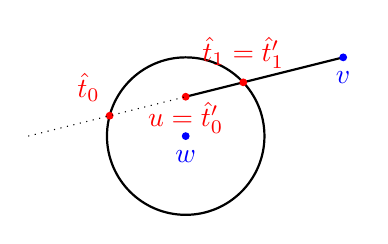
\begin{tikzpicture}
    % Define points
    \coordinate (u)  at (2,0.5);
    \coordinate (u0) at (0,0);
    \coordinate (v) at (4,1);
    \coordinate (w) at (2,0);

    % Draw the line segment from u to v
    \draw[thick] (u) -- (v);

    \draw[thick] (w) circle (1);

    % Find intersection points between the line and the circle
    \path[name path=line] (u0) -- (v);
    \path[name path=circle] (w) circle (1);
    \path[name intersections={of=line and circle, by={t1,t0}}];

    % Label intersection points
    \node[circle,fill,color=red,inner sep=1pt,label={[text=red, below]:\(u=\hat t_0'\)}] at (u) [] {}; 
    \node[circle,fill,color=blue,inner sep=1pt,label={[text=blue]-90:\(v\)}] at (v) [] {}; 
    \node[circle,fill,color=blue,inner sep=1pt,label={[text=blue]-90:\(w\)}] at (w) [] {}; 

    \node[circle,fill,color=red,inner sep=1pt,label={[text=red, above left]:\(\hat t_0\)}] at (t0) [] {}; 
    \node[circle,fill,color=red,inner sep=1pt,label={[text=red, above]:\(\hat t_1=\hat t_1'\)}] at (t1) [] {}; 

    % Draw dotted extensions of the line segment
    \draw[dotted] (u0) -- (u);
    %\draw[dotted] (v) -- ($(v)!-1.5!(u)$);
\end{tikzpicture}
\end{document}
